\documentclass[runningheads]{llncs}
\usepackage{graphicx}
%\usepackage[UKenglish]{babel}
%\usepackage[UKenglish]{isodate}
%\usepackage[utf8]{inputenc}
\usepackage[ruled,vlined]{algorithm2e}
\usepackage{amssymb}
\usepackage{mathtools}
\usepackage[capitalise]{cleveref}
\usepackage{tikz}
\usepackage{mathrsfs}
\usepackage[nounderscore]{syntax}
\usepackage{blkarray}

\usetikzlibrary{arrows.meta}

\newtheorem{constraint}{Constraint}

\renewcommand\fbox{\fcolorbox{red}{white}}

\newcommand{\variable}[1]{\texttt{\textup{#1}}}
\newcommand{\arrayd}[3]{\variable{{#1}[}{#2}\variable{]} \in {#3}}
\newcommand{\arrayt}[3]{\variable{{#3}[}{#2}\variable{] {#1}}}
\newcommand{\logical}[1]{{\normalfont \texttt{#1}}}

\newcommand{\predicates}{\mathcal{P}}
\newcommand{\variables}{\mathcal{V}}
\newcommand{\constants}{\mathcal{C}}
\newcommand{\tokens}{\mathcal{T}}
\newcommand{\arities}{\mathcal{A}}
\newcommand{\maxArity}{\mathcal{M}_{\mathcal{A}}}
\newcommand{\maxNumNodes}{\mathcal{M}_{\mathcal{N}}}
\newcommand{\maxNumClauses}{\mathcal{M}_{\mathcal{C}}}

\DeclareMathOperator{\Determined}{Determined}
\DeclareMathOperator{\Undetermined}{Undetermined}
\DeclareMathOperator{\AlmostDetermined}{AlmostDetermined}

%\relpenalty=10000
%\binoppenalty=10000
\def\multiset#1#2{\ensuremath{\left(\kern-.3em\left(\genfrac{}{}{0pt}{}{#1}{#2}\right)\kern-.3em\right)}}

\begin{document}

\title{Generating Random Logic Programs Using Constraint Programming}
\author{Paulius Dilkas\orcidID{0000-1111-2222-3333}}
\authorrunning{P. Dilkas}
% First names are abbreviated in the running head.
% If there are more than two authors, 'et al.' is used.

\institute{University of Edinburgh, Edinburgh, United Kingdom\\
  \email{p.dilkas@sms.ed.ac.uk}}
\maketitle

\begin{abstract}
The abstract should briefly summarize the contents of the paper in
150--250 words.

\keywords{Constraint Programming \and Logic Programming \and Probabilistic Logic
  Programming.}
\end{abstract}

\section{Introduction}

Motivation:
\begin{itemize}
\item Generating random programs that generate random data.
  %For example, enforcing that the decision is independent of gender.
\item Learning: how this can be used for (targeted) learning, when (atomic)
  probabilities can be assigned based on counting and we can have extra
  constraints. A more primitive angle: generate structures, learn weights.
\end{itemize}

TODO: define all the relevant terminology from logic and constraint programming.

If a predicate has arity $n$ and it is as of yet undecided what $n$ terms will
fill those spots, we will say that the predicate has $n$ \emph{gaps}. We say
that a constraint variable is \emph{(fully) determined} if its domain (at the
given moment in the execution) has exactly one value.

A \emph{(logic) program} is a multiset of clauses. Given a program
$\mathscr{P}$, a \emph{subprogram} $\mathscr{R}$ of $\mathscr{P}$ is a subset of
the clauses of $\mathscr{P}$ and is denoted by $\mathscr{R} \subseteq
\mathscr{P}$.

We will often use $\Box$ as a special domain value indicating a `disabled'
(i.e., fixed and ignored) part of the model. We write $\arrayd{a}{b}{c}$ to mean
that $\variable{a}$ is an array of variables of length $b$ such that each
element of $\variable{a}$ has domain $c$. Similarly, we write $\arrayt{a}{b}{c}$
to denote an array $\variable{a}$ of length $b$ such that each element of
$\variable{a}$ has type $\variable{c}$. All constraint variables in the model
are integer variables, but, e.g., if the integer $i$ refers to a logical
variable $X$, we will use $i$ and $X$ interchangeably. All indices start at
zero.

We also use Choco~4.10.2 \cite{choco}. This works with both Prolog
\cite{DBLP:books/daglib/0041598} and ProbLog \cite{DBLP:conf/ijcai/RaedtKT07}.
Tested with SWI-Prolog \cite{DBLP:journals/tplp/WielemakerSTL12}.

\subsection{Parameters}

Parameters:
\begin{itemize}
\item a list of predicates $\predicates{}$,
\item a list of their arities $\arities{}$ (including zero, but assuming that at
  least one predicate has non-zero arity),
  \begin{itemize}
  \item maximum arity $\maxArity{} \coloneqq \max \arities{}$.
  \end{itemize}
\item a list of variables $\variables{}$,
\item and a list of constants $\constants{}$.
  \begin{itemize}
  \item Each of them can be empty, but $|\constants{}| + |\variables{}| > 0$.
  \end{itemize}
\item a list of probabilities that are randomly assigned to clauses,
\item option to forbid all cycles or just negative cycles,
\item $\maxNumNodes{} \ge 1$: maximum number of nodes in the tree representation
  of a clause,
\item $\maxNumClauses{} \ge |\predicates{}|$: maximum number of clauses in a
  program,
\item maximum number of solutions,
\end{itemize}

We also define $\tokens{} = \{ \neg, \land, \lor, \top \}$. All decision
variables of the model are contained in two arrays:
\begin{itemize}
\item $\arrayt{bodiesOfClauses}{\maxNumClauses{}}{Body}$,
\item $\arrayt{headsOfClauses}{\maxNumClauses{}}{Head}$
\end{itemize}

\section{Heads of Clauses}

\begin{definition}
  The \emph{head} of a clause is composed of:
  \begin{itemize}
  \item a $\variable{predicate} \in \predicates \cup \{ \Box \}$.
  \item and $\arrayd{arguments}{\maxArity{}}{\constants{} \cup \variables{}}
    \cup \{ \Box \}$
  \end{itemize}
\end{definition}
The reason why $\Box$ must be a separate value will become clear in
\cref{sec:variable_symmetry}.

\begin{definition} \label{def:arity}
  The \variable{predicate}'s $\variable{arity} \in [0, \maxArity{}]$ can then be
  defined using the \variable{table} constraint as
  \[
    \variable{arity} = \begin{cases}
      \text{the arity of } \variable{predicate} & \text{if }
      \variable{predicate} \in \predicates{}\\
      0 & \text{otherwise.}
    \end{cases}
  \]
\end{definition}

\begin{constraint} \label{constr:arity}
  For $i = 0, \dots, \maxArity{} - 1$,
  \[
    \variable{arguments}[i] = \Box \iff i \ge \variable{arity}.
  \]
\end{constraint}

\section{Bodies of Clauses}

\begin{definition}
  The body of a clause is defined by:
  \begin{itemize}
  \item $\arrayd{treeStructure}{\maxNumNodes{}}{[0, \maxNumNodes{} - 1]}$ such
    that:
    \begin{itemize}
    \item $\variable{treeStructure}[i] = i$: the $i$-th node is a root.
    \item $\variable{treeStructure}[i] = j$: the $i$-th node's parent is node $j$.
    \end{itemize}
  \item $\arrayt{treeValues}{\maxNumNodes{}}{Node}$.
  \end{itemize}
\end{definition}

\begin{figure}[t]
  \centering
  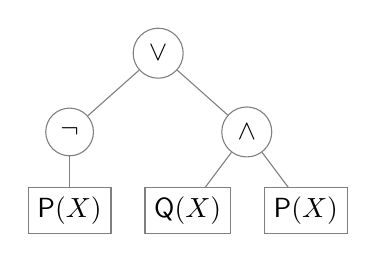
\begin{tikzpicture}
    \node[draw,circle,gray,text=black] (or) at (-0.375, 0) {$\lor$};
    \node[draw,circle,gray,text=black] (not) at (-1.5, -1) {$\neg$};
    \node[draw,circle,gray,text=black] (and) at (0.75, -1) {$\land$};
    \node[draw,gray,text=black] (P) at (-1.5, -2) {$\mathsf{P}(X)$};
    \node[draw,gray,text=black] (Q) at (0, -2) {$\mathsf{Q}(X)$};
    \node[draw,gray,text=black] (R) at (1.5, -2) {$\mathsf{P}(X)$};
    \draw[gray] (or) -- (not);
    \draw[gray] (or) -- (and);
    \draw[gray] (not) -- (P);
    \draw[gray] (and) -- (Q);
    \draw[gray] (and) -- (R);
  \end{tikzpicture}
  \caption{A tree representation of the formula from \cref{example:formula}}
  \label{fig:example_tree}
\end{figure}

\begin{example} \label{example:formula}
  Let $\maxNumNodes{} = 8$. Then $\neg\mathsf{P}(X) \lor (\mathsf{Q}(X)
  \land \mathsf{P}(X))$ corresponds to the tree in \cref{fig:example_tree} and
  can be encoded as:
  \begin{alignat*}{8}
    \variable{treeStructure} &= [0, &&0, &&0, &&1, &&2, &&2, &&6, &&7],\\
    \variable{treeValues} &= [{\lor}, &&{\neg}, &&{\land}, \mathsf{P}(&&X), \mathsf{Q}(&&X), \mathsf{P}(&&X), &&\top, &&\top],\\
    \variable{numNodes} &= 6, && && && && && && &&\\
    \variable{numTrees} &= 3. && && && && && && &&
  \end{alignat*}
  In the rest of this section, we will describe how the elements of
  $\variable{treeValues}$ are encoded and list a series of constraints that make
  this representation unique.
\end{example}

\subsection{Nodes}

\begin{definition} \label{def:node}
  A \emph{node} has a $\variable{name} \in \tokens{} \cup \predicates{}$ and
  $\arrayd{arguments}{\maxArity{}}{\variables{} \cup \constants{} \cup \{ \Box
    \}}$. The node's $\variable{arity}$ can then be
  defined analogously to \cref{def:arity}.
\end{definition}

We can use \cref{constr:arity} again to disable extra arguments.

\begin{example}
  Let $\maxArity{} = 2$, $\predicates{} = [\mathsf{P}, \dots]$, $\arities{}
  = [1, \dots]$, and $X \in \variables{}$. Then the node representing atom
  $\mathsf{P}(X)$ has:
  \begin{align*}
    \variable{name} &= \mathsf{P},\\
    \variable{arguments} &= [X, \Box],\\
    \variable{arity} &= 1.
  \end{align*}
\end{example}

\subsection{Constraints}

\begin{definition}
  We define $\variable{numTrees} \in \{ 1, \dots, \maxNumNodes{} \}$ to count
  the number of trees in our representation of a clause using the
  $\variable{tree}(\variable{treeStructure}, \variable{numTrees})$\footnote{This
    constraint uses dominator-based filtering by Fages and Lorca
    \cite{DBLP:conf/cp/FagesL11}.} constraint.
\end{definition}

\begin{definition}
  For convenience, we also define $\variable{numNodes} \in \{ 1, \dots,
  \maxNumNodes{} \}$ to count the number of nodes in the main tree. We define it
  as
  \[
    \variable{numNodes} = \maxNumNodes{} - \variable{numTrees} + 1.
  \]
\end{definition}

\begin{constraint}
  $\variable{treeStructure}[0] = 0$.
\end{constraint}

\begin{constraint}
  \variable{treeStructure} is sorted.
\end{constraint}

\begin{constraint}
  For $i = 0, \dots, \maxNumNodes{} - 1$, if $\variable{numNodes} \le
  i$, then
  \[
    \variable{treeStructure}[i] = i \quad \text{and} \quad
    \variable{treeValues}[i].\variable{name} = \top,
  \]
  else
  \[
    \variable{treeStructure}[i] < \variable{numNodes}.
  \]
\end{constraint}

\begin{constraint}
  For $i = 0, \dots, \maxNumNodes{} - 1$,
  \begin{align*}
    \variable{count}(i, \variable{treeStructure}_{-i}) = 0 &\iff \variable{treeValues}[i].\variable{name} \in \predicates{} \cup \{ \top \},\\
    \variable{count}(i, \variable{treeStructure}_{-i}) = 1 &\iff \variable{treeValues}[i].\variable{name} = \neg,\\
    \variable{count}(i, \variable{treeStructure}_{-i}) > 1 &\iff \variable{treeValues}[i].\variable{name} \in \{ \land, \lor \},
  \end{align*}
  where $\variable{treeStructure}_{-i}$ denotes array $\variable{treeStructure}$
  with position $i$ skipped.
\end{constraint}
Each constraint corresponds to node $i$ having no children, one child, and
multiple children, respectively.


\begin{constraint}
  For $i = 0, \dots, \maxNumNodes{} - 1$,
  \[
    \variable{treeStructure}[i] \ne i \implies
    \variable{treeValues}[i].\variable{name} \ne \top.
  \]
\end{constraint}

\begin{constraint}
  For $i = 0, \dots, \maxNumClauses{} - 1$, if
  $\variable{headsOfClauses}[i].\variable{predicate} = \Box$, then
  \[
    \variable{bodiesOfClauses}[i].\variable{numNodes} = 1,
  \]
  and
  \[
    \variable{bodiesOfClauses}[i].\variable{treeValues}[0].\variable{name} =
    \top.
  \]
\end{constraint}

\section{Eliminating Variable Symmetries} \label{sec:variable_symmetry}

Given any clause, we can permute the variables in it without changing the
meaning of the clause or the entire program. Thus, we want to fix the order of
variables to eliminate unnecessary symmetries. Informally, we can say that
variable $X$ goes before variable $Y$ if its first occurrence in either the head
or the body of the clause is before the first occurrence of $Y$. Note that the
constrains described in this section only make sense if $|\variables| > 1$. Also
note that all definitions and constraints here are on a per-clause basis.

\begin{definition}
  Let $N = \maxArity{} \times (\maxNumNodes{} + 1)$. Let
  $\variable{terms}[N] \in \constants{} \cup \variables{} \cup \{ \Box
  \}$ be a flattened array of all gaps in a particular clause.

  Then we can use the $\variable{setsIntsChanneling}$ constraint
  to define $\variable{occurrences}[|\constants{}| + |\variables{}| + 1]$ as an
  array of subsets of $\{ 0, \dots, N-1 \}$ such that for all $i = 0, \dots, N
  - 1$, and $t \in \constants{} \cup \variables{} \cup \{ \Box \}$,
  \[
    i \in \variable{occurrences}[t] \quad \iff \quad
    \variable{terms}[i] = t
  \]
\end{definition}

\begin{definition}
  We define $\arrayd{introductions}{|\variables{}|}{\{ 0, \dots, N \}}$ such
  that for $v \in \variables{}$,
  \[
    \variable{introductions}[v] = \begin{cases}
      1 + \min \variable{occurrences}[v] & \text{if }
      \variable{occurrences}[v] \ne \emptyset\\
      0 & \text{otherwise.}
    \end{cases}
  \]
\end{definition}

\begin{constraint}
  $\variable{introductions}$ are sorted.
\end{constraint}

\begin{example}
  Let $\constants{} = \emptyset$, $\variables{} = \{ X, Y, Z \}$, $\maxArity{} =
  2$, $\maxNumNodes{} = 3$, and consider the clause
  \[
    \mathsf{sibling}(X, Y) \gets \mathsf{parent}(X, Z) \land
    \mathsf{parent}(Y, Z).
  \]
  Then $\variable{terms} = [X, Y, \Box, \Box, X, Z, Y, Z]$ (the boxes represent
  the conjunction node), $\variable{occurrences} = [\{ 0, 4 \}, \{ 1, 6 \},
  \{ 5, 7 \}, \{ 2, 3 \}]$, and $\variable{introductions} = [0, 1, 5]$.
\end{example}

\subsection{Redundant Constraints}
% TODO: need writing. For example: why do I need them?

\begin{constraint}
  For $u \ne v \in \constants{} \cup \variables{} \cup \{ \Box \}$,
  \[
    \variable{occurrences}[u] \cap \variable{occurrences}[v] = \emptyset.
  \]
\end{constraint}

\begin{constraint}
  $\variable{allDifferentExcept0}(\variable{introductions})$.
\end{constraint}

\begin{constraint}
  For $v \in \variables{}$,
  \[
    \variable{introductions}[v] \ne 0 \quad \implies \quad
    \variable{introductions}[v] - 1 \in \variable{occurrences}[v].
  \]
\end{constraint}

\begin{definition}
  We define an auxiliary set variable
  \[
    \variable{potentialIntroductions} \subseteq \{ 0, \dots, N \}
  \]
  by: for $i = 0, \dots, \maxNumNodes{} - 1$, if
  $\variable{treeValues}[i].\variable{name} \in \tokens{}$, then
  \[
    \variable{potentialIntroductions} \cap \{ \maxArity{} \times (i + 1) + j + 1
    \mid j = 0, \dots, \maxArity{} - 1 \} = \emptyset.
  \]
\end{definition} % TODO: maybe add to the example
In other words, if the node not a predicate, a variable cannot be introduced as
one of its `arguments'.

\begin{constraint}
  For $v \in \variables{}$, $\variable{introductions}[v] \in
  \variable{potentialIntroductions}$.
\end{constraint}

\section{Interactions Between Clauses}

\begin{constraint}
  Each predicate gets at least one clause. Let
  \[
    P = \{ h.\variable{predicate} \mid h \in \variable{headsOfClauses} \}.
  \]
  Then
  \[
    \variable{nValues}(P) =
    \begin{cases}
      \variable{numPredicates} + 1 & \text{if } \variable{count}(\Box, P) > 0 \\
      \variable{numPredicates} & \text{otherwise.}
    \end{cases}
  \]
  Here, $\variable{nValues}(P)$ counts the number of unique values in $P$.
\end{constraint}

\begin{constraint}
  Clauses are sorted.
\end{constraint}

\section{Counting Programs}

In order to demonstrate the correctness of the model and explain it in more
detail, in this section we are going to derive combinatorial expressions for
counting the number of programs with up to $\maxNumClauses{}$ clauses and up to
$\maxNumNodes{}$ nodes per clause, and arbitrary $\predicates{}$,
$\arities{}$, $\variables{}$, and $\constants{}$. To simplify the task, we only
consider clauses without probabilities and disable (negative) cycle elimination.
It was experimentally confirmed that the model agrees with the combinatorial
formula from this section in 985 different scenarios. The \emph{total arity} of
a body of a clause is the sum total of arities of all predicates in the body.

We will first consider clauses with gaps, i.e., without taking variables and
constants into account. Let $T(n, a)$ denote the number of possible clause
bodies with $n$ nodes and total arity $a$. Then $T(1, a)$ is the number of
predicates in $\predicates{}$ with arity $a$, and the following recursive
definition can be applied for $n > 1$:
\[
  T(n, a) = T(n-1, a) + 2\sum_{\substack{c_1 + \dots + c_k = n - 1,\\
      2 \le k \le \frac{a}{\min \arities{}},\\
      c_i \ge 1 \text{ for all } i}} \sum_{\substack{d_1 + \dots + d_k = a,\\
    d_i \ge \min \arities{} \text{ for all } i}} \prod_{i=1}^k T(c_i, d_i).
\]
The first term here represents negation, i.e., negating an expression consumes
one node but otherwise leaves the task unchanged. If the first operation is not
negation, then it must be either conjunction or disjunction (hence the
coefficient `2'). In the first sum, $k$ represents the number of children of the
root node, and each $c_i$ is the number of nodes dedicated to child $i$. Thus,
the first sum iterates over all possible ways to partition the remaining $n-1$
nodes. Similarly, the second sum considers every possible way to partition the
total arity $a$ across the $k$ children nodes.

We can then count the number of possible clause bodies with total arity $a$ (and
any number of nodes) as
\[
  C(a) = \begin{cases}
    1 & \text{if } a = 0\\
    \sum_{n=1}^{\maxNumNodes{}} T(n, a) & \text{otherwise.}
  \end{cases}
\]
Here, the empty clause is considered separately.

The number of ways to fill $n$ gaps with terms can be expressed as
\[
  P(n) = |\constants{}|^n + \sum_{\substack{1 \le k \le |\variables{}|, \\ 0 =
      s_0 < s_1 < \dots < s_k < s_{k+1} = n+1}} \prod_{i=0}^k (|\constants{}| +
  i)^{s_{i+1} - s_i - 1}.
\]
The first term is simply the number of ways to fill all $n$ gaps with
constants. The parameter $k$ is the number of variables used in the clause, and
$s_1, \dots, s_k$ mark the first occurrence of each variable. For each gap
between any two introductions (or before the first introduction, or after the last
introduction), we have $s_{i+1}-s_i-1$ spaces to be filled with any of the
$\constants{}$ constants or any of the $i$ already-introduced variables.

Let us order the elements of $\predicates{}$, and let $a_i$ be the arity of the
$i$-th predicate. The number of programs is then:
\[
  \sum_{\substack{ \sum_{i=1}^{|\predicates{}|} h_i = n,\\
      |\predicates{}| \le n \le \maxNumClauses,\\
      h_i \ge 1 \text{ for all } i}} \prod_{i=1}^{|\predicates{}|}
  \multiset{\sum_{a=0}^{\maxArity{} \times \maxNumNodes{}} C(a) P(a+a_i)}{h_i},
\]
where
\[
  \multiset{n}{k} = \binom{n+k-1}{k}
\]
counts the number of ways to select $k$ out of $n$ items with repetition (and
without ordering). Here, we sum over all possible ways to distribute
$|\predicates{}| \le n \le \maxNumClauses{}$ clauses among $|\predicates{}|$
predicates so that each predicate gets at least one clause. For each predicate,
we can then count the number of ways to select its clauses out of all possible
clauses. The number of possible clauses can be computed by considering each
possible arity $a$, and multiplying the number of `unfinished' clauses $C(a)$ by
the number of ways to fill the $a+a_i$ gaps in the body and the head of the
clause with terms.

\section{Predicate Independence}

In this section, we define a notion of predicate independence as a way to
constrain the probability distributions defined by the generated programs. We
also describe efficient algorithms for propagation and entailment checking.

\begin{definition}
  Let $\mathscr{P}$ be a probabilistic logic program. Its \emph{predicate
    dependency graph} is a directed graph $G_{\mathscr{P}} = (V, E)$ with the
  set of nodes $V$ consisting of all predicates in $\mathscr{P}$. For any two
  different predicates $\mathsf{P}$ and $\mathsf{Q}$, we add an edge from
  $\mathsf{P}$ to $\mathsf{Q}$ if there is a clause in $\mathscr{P}$ with
  $\mathsf{Q}$ as the head and $\mathsf{P}$ mentioned in the body. We say that
  the edge is \emph{negative} if there exists a clause with $\mathsf{Q}$ as the
  head and at least one instance of $\mathsf{P}$ at the body such that the path
  from the root to the $\mathsf{P}$ node in the tree representation of the
  clause passes through at least one negation node. Otherwise it is
  \emph{positive}. We say that $\mathscr{P}$ (or $G_{\mathscr{P}}$) has a
  \emph{negative cycle} if $G_{\mathscr{P}}$ has a cycle with at least one
  negative edge.
\end{definition}

\begin{definition}
  Let $\mathsf{P}$ be a predicate in a program $\mathscr{P}$. The
  \emph{dependencies} of $\mathsf{P}$ is the smallest set $D_{\mathsf{P}}$ such
  that:
  \begin{itemize}
  \item $\mathsf{P} \in D_{\mathsf{P}}$,
  \item for every $\mathsf{Q} \in D_{\mathsf{P}}$, the nodes with arrows to
    $\mathsf{Q}$ in $G_{\mathscr{P}}$ are all in $D_{\mathsf{P}}$.
  \end{itemize}
\end{definition}

\begin{definition}
  Two predicates $\mathsf{P}$ and $\mathsf{Q}$ are \emph{independent} if
  $D_{\mathsf{P}} \cap D_{\mathsf{Q}} = \emptyset$.
\end{definition}

\begin{figure}[t]
  \centering
  \begin{minipage}{.5\textwidth}
    \centering
    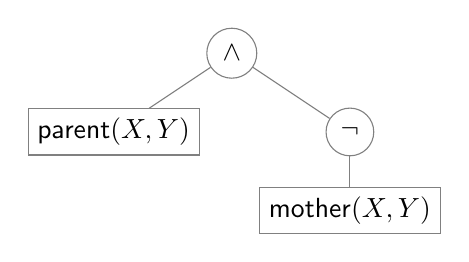
\begin{tikzpicture}
      \node[draw,circle,gray,text=black] (and) at (0, 0) {$\land$};
      \node[draw,circle,gray,text=black] (not) at (1.5, -1) {$\neg$};
      \node[draw,gray,text=black] (parent) at (-1.5, -1) {$\mathsf{parent}(X, Y)$};
      \node[draw,gray,text=black] (mother) at (1.5, -2) {$\mathsf{mother}(X, Y)$};
      \draw[gray] (and) -- (parent);
      \draw[gray] (and) -- (not);
      \draw[gray] (not) -- (mother);
    \end{tikzpicture}
    \caption{The tree representation of the body of Clause~\eqref{eq:example_clause}.}
    \label{fig:example_tree2}
  \end{minipage}
  \begin{minipage}{.49\textwidth}
    \centering
    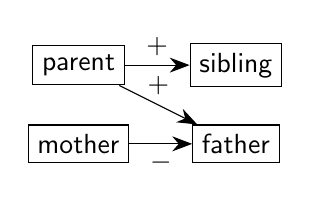
\begin{tikzpicture}
      \node[draw] (parent) at (0, 0.5) {$\mathsf{parent}$};
      \node[draw] (mother) at (0, -0.5) {$\mathsf{mother}$};
      \node[draw] (sibling) at (2, 0.5) {$\mathsf{sibling}$};
      \node[draw] (father) at (2, -0.5) {$\mathsf{father}$};
      \draw[-{Stealth[scale=1.5]}] (parent) edge node[above] {$+$} (sibling);
      \draw[-{Stealth[scale=1.5]}] (parent) edge node[above] {$+$} (father);
      \draw[-{Stealth[scale=1.5]}] (mother) edge node[below] {$-$} (father);
    \end{tikzpicture}
    \caption{The predicate dependency graph of the program in \cref{ex:program}.
      Positive edges are labeled with `$+$', and negative edges with `$-$'.}
    \label{fig:predicate_dependencies}
  \end{minipage}
\end{figure}

% TODO: example of edge positivity/negativity
% TODO: this is not a complete program (by my definition). Make it clear in the text.
\begin{example} \label{ex:program}
  Consider the following program:
  \begin{align}
    \mathsf{sibling}(X, Y) &\gets \mathsf{parent}(X, Z) \land \mathsf{parent}(Y, Z), \nonumber \\
    \mathsf{father}(X, Y) &\gets \mathsf{parent}(X, Y) \land \neg\mathsf{mother}(X, Y). \label{eq:example_clause}
  \end{align}
  Its predicate dependency graph is in \cref{fig:predicate_dependencies}.
  Because of the negation in \cref{eq:example_clause} (as seen in
  \cref{fig:example_tree2}), the edge from $\mathsf{mother}$ to
  $\mathsf{father}$ is negative, while the other two edges are positive.

  We can now list the dependencies of each predicate:
  \begin{alignat*}{3}
    D_{\mathsf{parent}} &= \{ \mathsf{parent} \}, \quad && D_{\mathsf{sibling}}
    &&= \{\mathsf{sibling}, \mathsf{parent} \},\\
    D_{\mathsf{mother}} &= \{ \mathsf{mother} \}, \quad && D_{\mathsf{father}}
    &&= \{ \mathsf{father}, \mathsf{mother}, \mathsf{parent} \}.
  \end{alignat*}
  Hence, we have two pairs of independent predicates, i.e., $\mathsf{mother}$ is
  independent from $\mathsf{parent}$ and $\mathsf{sibling}$.
\end{example}

\begin{definition}[Adjacency matrix representation] \label{def:adjacency_matrix}
  An $|\predicates{}| \times |\predicates{}|$ adjacency matrix $\mathbf{A}$ with
  $\{ 0, 1 \}$ as its domain is defined by
  \begin{align*}
    \mathbf{A}[i][j] = 0 \iff &\nexists k \in \{ 0, \dots, \maxNumClauses{} \}: \variable{headsOfClauses}[k].\variable{predicate} = j \text{ and } \\
    &i \in \{ a.\variable{name} \mid a \in \variable{bodiesOfClauses}[k].\variable{treeValues} \}.
  \end{align*}
\end{definition}

% TODO: continue writing from here
We define a \emph{dependency} as an algebraic data type that is either
determined (in which case it holds only the index of the \texttt{predicate}) or
undetermined (in which case it also holds the indices of the \texttt{source} and
\texttt{target} vertices, corresponding to the edge responsible for making the
dependency undetermined (exactly one, otherwise we don't consider the edge)).

Propagation for independence:
\begin{itemize}
\item Look up the dependencies of both predicates. For each pair of
  matching dependencies:
  \begin{itemize}
  \item If both are determined, fail.
  \item If one is determined, the selected edge of the other must not
    exist.
  \end{itemize}
\end{itemize}

\begin{algorithm}[p]
  \SetKwFunction{getDependencies}{getDependencies}
  \SetKwFunction{isDetermined}{isDetermined}
  \SetKwFunction{fail}{fail}
  \SetKwFunction{removeValue}{removeValue}
  \SetKwData{predicate}{predicate}
  \SetKwData{source}{source}
  \SetKwData{target}{target}
  \KwData{predicates $p_1$, $p_2$; adjacency matrix $\mathbf{A}$}
  \For{$(d_1, d_2) \in \getDependencies{$p_1$, \logical{false}} \times
      \getDependencies{$p_2$, \logical{false}}$ such that $d_1.\predicate =
      d_2.\predicate$}{
    \lIf{$d_1$ {\bf is} $\Determined$ {\bf and} $d_2$ {\bf is}
      $\Determined$}{\fail{}}
    \If{$d_1$ {\bf is} $\Determined$ {\bf and} $d_2$ {\bf is}
      $\AlmostDetermined(\_, s, t)$ {\bf or} \hspace{50pt} $d_2$ {\bf is} $\Determined$ {\bf
        and} $d_1$ {\bf is} $\AlmostDetermined(\_, s, t)$}{
      $\mathbf{A}[s][t]$.\removeValue{$1$}\;
    }
  }
  \caption{Propagation algorithm for predicate independence}
\end{algorithm}

\begin{algorithm}[p]
  \SetKwFunction{getDependencies}{getDependencies}
  \SetKwFunction{isDetermined}{isDetermined}
  \SetKwData{predicate}{predicate}
  \KwData{predicates $p_1$, $p_2$}
  $D \gets \{ (d_1, d_2) \in \getDependencies{$p_1$, \logical{true}} \times
  \getDependencies{$p_2$, \logical{true}} \mid d_1.\predicate = d_2.\predicate
  \}$\;
  \lIf{$D = \emptyset$}{\Return{\textsc{true}}}
  \lIf{$\exists (\Determined \_, \Determined \_) \in D$}{\Return{\textsc{false}}}
  \Return{\textsc{undefined}}\;
  \caption{Entailment check for predicate independence}
  \label{alg:independence_entailment}
\end{algorithm}

% TODO: introduce this sum data type syntax
\begin{grammar}
  <dependency> ::= $\Determined p$ | $\Undetermined p$ | $\AlmostDetermined(p, s, t)$
\end{grammar}
where $p,s,t \in \predicates{}$. For a dependency $d$---regardless of its exact
type---we will refer to its predicate $p$ as $d.\variable{predicate}$.
% TODO: underscore represents a variable that can take any value (different
% underscores can take different values)

\begin{algorithm}[p]
  \SetKwData{edgeExists}{edgeExists}
  \SetKwData{predicate}{predicate}
  \SetKwData{source}{source}
  \SetKwData{target}{target}
  \SetKwData{all}{allDependencies}
  \SetKwFunction{isDetermined}{isDetermined}
  \SetKwFunction{getDependencies}{getDependencies}
  \SetKwProg{Fn}{Function}{:}{}
  \KwData{a $|\predicates{}| \times |\predicates{}|$ adjacency matrix
    $\mathbf{A}$ with $\{ 0, 1 \}$ as the domain}
  \Fn{\getDependencies{$p$, \all}} {
    $D \gets \{ \Determined p \}$\;
    \While{\logical{true}}{
      $D' \gets \emptyset$\;
      \For{$d \in D$ {\bf and} $q \in \predicates{}$}{
        $\edgeExists \gets \mathbf{A}[q][d.\predicate] = \{ 1 \}$\;
        \uIf{$\edgeExists$ {\bf and} $d$ {\bf is} $\Determined$}{
          $D' \gets D' \cup \{ \Determined q \}$
        }
        \uElseIf{$\edgeExists$ {\bf and} $d$ {\bf is} $\AlmostDetermined(\_, s, t)$}{
          $D' \gets D' \cup \{ \AlmostDetermined(q, s, t) \}$\;
        }
        \uElseIf{$|\mathbf{A}[q][d.\predicate]| > 1$ {\bf and} $d$ {\bf is}
          $\Determined r$}{
          $D' \gets D' \cup \{ \AlmostDetermined(q, q, r) \}$\;
        }
        \ElseIf{$|\mathbf{A}[q][d.\predicate]| > 1$ {\bf and} \all}{
          $D' \gets D' \cup \{ \Undetermined q \}$\;
        }
      }
      \lIf{$D' = D$}{\Return{$D$}}
      $D \gets D'$\;
    }
  }
  \caption{Computing the dependencies of a predicate}
\end{algorithm}
% TODO: any way to test all of this?

% TODO: Discuss that the algorithms work in case there are multiple 'paths'
% without any issues.

\begin{figure}[t]
  \centering
  \begin{minipage}{.49\textwidth}
    \centering
    \[
      \begin{blockarray}{ccccccc}
        \begin{block}{ccc(cccc)}
          \mathsf{father} & & & 0 & 0 & 0 & 0 \\
          \mathsf{mother} & & & 1 & 0 & 0 & 0 \\
          \mathsf{parent} & & & 1 & \fbox{\{ 0, 1 \}} & \{ 0, 1 \} & \{ 0, 1 \} \\
          \mathsf{sibling} & & & 0 & 0 & 0 & 0 \\
        \end{block}
      \end{blockarray}
    \]
    \caption{The adjacency matrix defined using \cref{def:adjacency_matrix} for
      \cref{example:independence}}
    \label{fig:dependencies_matrix}
  \end{minipage}
  \begin{minipage}{.5\textwidth}
    \centering
    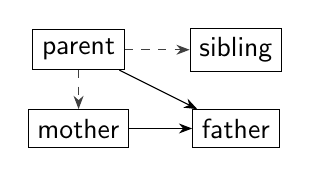
\begin{tikzpicture}
      \node[draw] (parent) at (0, 0.5) {$\mathsf{parent}$};
      \node[draw] (mother) at (0, -0.5) {$\mathsf{mother}$};
      \node[draw] (sibling) at (2, 0.5) {$\mathsf{sibling}$};
      \node[draw] (father) at (2, -0.5) {$\mathsf{father}$};
      \draw[-{Stealth}] (parent) edge (father);
      \draw[-{Stealth}] (mother) edge (father);
      \draw[-{Stealth},dashed,darkgray] (parent) edge (sibling);
      \draw[-{Stealth},dashed,darkgray] (parent) edge (mother);
    \end{tikzpicture}
    \caption{The predicate dependency graph that corresponds to
      \cref{fig:dependencies_matrix}. Dashed edges are undetermined---they may
      or may not exist.}
    \label{fig:dependencies2}
  \end{minipage}
\end{figure}
% TODO: make sure my definitions and examples are consistent with loops

\begin{example} \label{example:independence}
  Consider this partially determined (fragment of a) program:
  \begin{align*}
    \Box(X, Y) &\gets \mathsf{parent}(X, Z) \land \mathsf{parent}(Y, Z),\\
    \mathsf{father}(X, Y) &\gets \mathsf{parent}(X, Y) \land \neg\mathsf{mother}(X, Y)
  \end{align*}
  where $\Box$ indicates an unknown predicate with domain
  \[
    D = \{ \mathsf{father}, \mathsf{mother}, \mathsf{parent}, \mathsf{sibling}
    \}.
  \]
  The predicate dependency graph (without positivity/negativity) defined by
  \cref{def:adjacency_matrix} is represented in
  \cref{fig:dependencies_matrix,fig:dependencies2}.

  Suppose we have a constraint that $\mathsf{mother}$ and $\mathsf{parent}$ must
  be independent. The lists of potential dependencies for both predicates are:
  \begin{align*}
    D_{\mathsf{mother}} &= \{ \Determined \mathsf{mother}, \AlmostDetermined(\mathsf{parent}, \mathsf{parent}, \mathsf{mother}) \}, \\
    D_{\mathsf{parent}} &= \{ \Determined \mathsf{parent} \}.
  \end{align*}
  An entailment check at this stage would produce \textsc{undefined}, but
  propagation replaces the boxed value in \cref{fig:dependencies_matrix} with
  zero, eliminating the potential edge from $\mathsf{parent}$ to
  $\mathsf{mother}$. This also eliminates $\mathsf{mother}$ from $D$, and,
  although some undetermined variables remain, this is enough to make
  \cref{alg:independence_entailment} return \textsc{true}.
\end{example}

\section{Entailment Checking for Negative/All Cycles}
% TODO: explain that the hasNegativeCycles algorithm is an extension of a simple
% cycle detection algorithm.
% TODO: the difficulty with propagation is that there is no good way to define
% the adjacency matrix with 0/-1/+1 values, the negativity condition is too
% difficult.
% TODO: NB: the set of decision variables for this constraint must exclude all
% arguments.
% In order to avoid thrashing, we fix the following variable ordering: [...]. Example of thrashing: P(X, a) <- ~P(X, b) contradicts the negative cycle constrant. Let's try P(X, a) <- P(X, c) instead (and so on).

\begin{algorithm}[t]
  \KwData{a constraint model for a logic program $\mathscr{P}$ amid execution}
  \SetKwFunction{hasNegativeCycles}{hasNegativeCycles}
  Let $\mathscr{R} \subseteq \mathscr{P}$ be the largest subprogram of
  $\mathscr{P}$ with all bodies and all predicates in heads fully
  determined\footnotemark\;
  \lIf{$\mathscr{R} = \emptyset$}{\Return{\textsc{undefined}}}
  \lIf{\hasNegativeCycles($G_{\mathscr{R}}$)}{\Return{\textsc{false}}}
  \lIf{$\mathscr{R} = \mathscr{P}$}{\Return{\textsc{true}}}
  \Return{\textsc{undefined}}\;
  \caption{Entailment check for negative cycles}
\end{algorithm}
\footnotetext{Due to the definition of independence, the arguments of the head
  atom need not be determined.}

\section{Experimental Results}

\section{Conclusion \& Future Work}

\begin{itemize}
\item A constraint for logical equivalence. An algorithm to reduce each tree to
  some kind of normal form. Not doing this on purpose. Leaving for further work.
\item Perhaps negative cycle detection could use the same graph as the
  independence propagator? If we extend each domain to {-1, 0, 1}, but that
  might make propagation weaker or slower.
\item Could investigate how uniform the generated distribution of programs is.
  Distributions of individual parameters will often favour larger values
  because, e.g., there are more 5-tuples than 4-tuples.
\item Inference options to explore. Logspace vs normal space. Symbolic vs
  non-symbolic. Propagate evidence (might be irrelevant)? Propagate weights?
  Supported knowledge compilation techniques: sdd, sddx, bdd, nnf, ddnnf, kbest,
  fsdd, fbdd.
\item Mention the random heuristic. Mention that restarting gives better
  randomness, but duplicates become possible. Restarting after each run is
  expensive. Periodic restarts could be an option.
\item Could add statistics about what constraints tend to conflict.
\end{itemize}

\section*{Acknowledgments}

% The author would like to thank Vaishak Belle for his comments.
This work was supported by the EPSRC Centre for Doctoral Training in Robotics
and Autonomous Systems, funded by the UK Engineering and Physical Sciences
Research Council (grant EP/S023208/1).

\bibliographystyle{splncs04}
\bibliography{paper}

\end{document}